\section*{Aufgabe 2: BFGS-Verfahren}

Mit Hilfe des BFGS-Verfahrens kann ein mehrdimensionales Nullstellen Problem einer Funktion $f(x_1,x_2...,x_N)$ mit Aufwand $\mathcal{O}(N^2)$ gelöst werden kann.
Dazu wird eine inverse Hesse-Matrix $C_0$ initialisiert und über die folgende Form die Iterationen bestimmt:
\begin{align*}
C_{k+1} &= (\mathds{1} - \underbrace{\frac{1}{\vec{s}_k^T\vec{y}_k}}_{=:\rho}\vec{s}_k\vec{y}_k^T)C_k(\mathds{1}-\frac{1}{\vec{s}_k^T\vec{y}_k}\vec{y}_k\vec{s}_k^T) +\frac{1}{\vec{s}_k^T\vec{y}_k}\vec{s}_k\vec{s}_k^T\\
&= C_k - \rho ((C_k\vec{y}_k)\vec{s}_k^T + \vec{s}_k(\vec{y}_k^TC_k)) + \rho^2\vec{s}_k(\vec{y}_k^T(C_k\vec{y}_k))\vec{s}_k^T +\rho\vec{s}_k\vec{s}_k^T
\end{align*}
Dabei sind
\begin{align*}
\vec{y}_k &= \vec{b}_{k+1} - \vec{b}_k = -\nabla(f(\vec{x}_{k+1})-f(\vec{x}_{k+1}))\\
\vec{s}_k &= \vec{x}_{k+1} - \vec{x}_k = C_k \vec{b_{k}}
\end{align*}
\subsection*{c)}
\label{sec:c}
Die Matrix $C_0$ zum Problem aus Gleichung\eqref{eq:1} mit dem Startvektor
\[
\vec{x}_0 = \begin{pmatrix}
-1\\
1
\end{pmatrix}
\]
wird auf drei verschiedene Arten initialisiert:
\begin{enumerate}
\item Die exakte inverse Hesse-Matrix.
\item Eine Diagonalmatrix mit den inversen Hauptdiagonalelementen der Hesse-Matrix.
\item Eine Diagonalmatrix in der Größenordnung von $f$.
\end{enumerate}
Beim letzten Punkt wurde hier $C_0 = \frac{1}{f(\vec{x}_0}\mathds{1}$ gesetzt.
Die Entwicklung der Gradientennorm $|\vec{b}_k|$ in Abhängigkeit vom Iterationsschritt $k$ für die drei verschiedenen Startmatrizen bis zu einer Genauigkeit $\epsilon < 10^{-5}$ ist in Abbildung \ref{fig:1} zu sehen. Dabei benötigt erstaunlicherweise die exakte Hesse-Matrix die meisten Iterationsschritte. Es zeigt sich außerdem, dass es besonders für Methode 1. und 3. zu starken Ausreißern in der Gradientennorm kommt, sodass sich der Algorithmus wieder vom Minimum 
\[
\hat{\vec{x}} = \begin{pmatrix}
1 \\
1
\end{pmatrix}
\]
entfernt (s.Abb.\ref{fig:2}).
Dies kann verbessert werden indem nach jedem Schritt des BFGS-Verfahrens ein weiterer Liniensuchschritt durchgeführt wird um ein sinnvolles $\vec{s}_k = \lambda C_k \vec{b_{k}}$ zu finden.
Die zugehörigen Gradientennorm und der Abstand zum Minimum in Abhängigkeit vom Iterationsschritt sind in Abbildung\ref{fig:3} und \ref{fig:4} abgebildet.
Es zeigt sich, dass
\begin{figure}
\centering
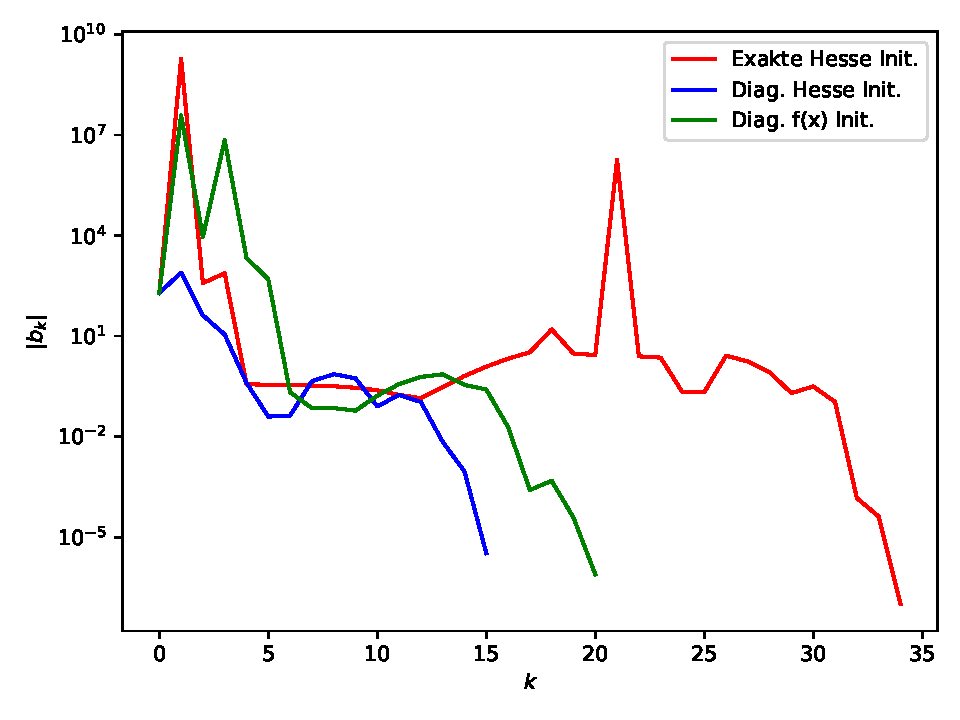
\includegraphics[width=0.45\textwidth]{A2/build/A2.pdf}
\caption{$|b_k|$ in Abhängigkeit vom Iterationschritt.}
\label{fig:1}
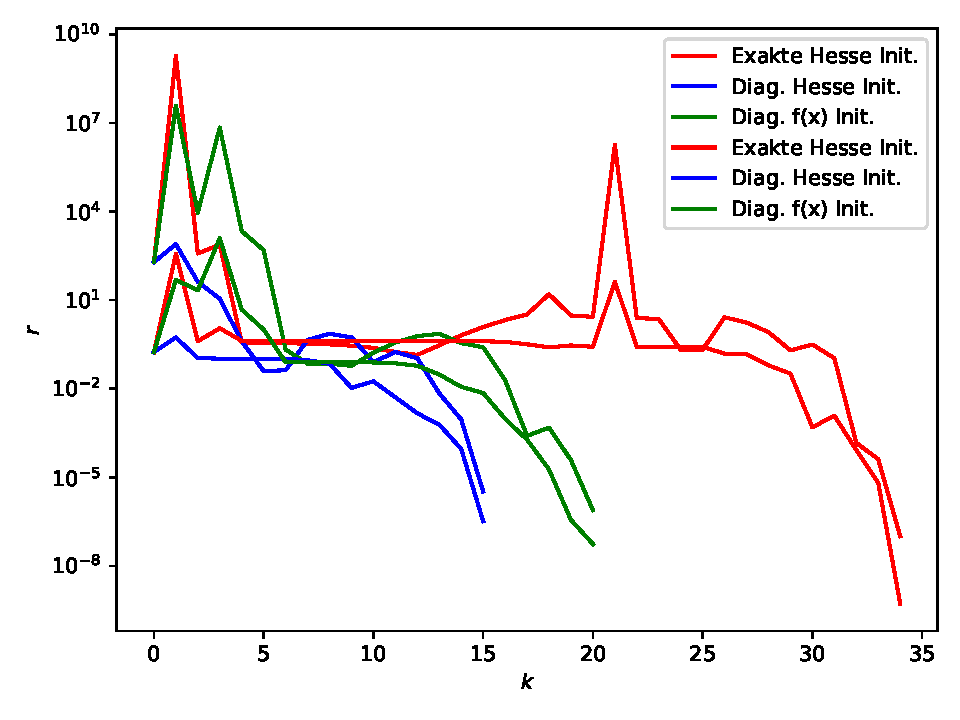
\includegraphics[width=0.45\textwidth]{A2/build/A2r.pdf}
\caption{Abweichung zum Minimum in Abhängigkeit vom Iterationschritt.}
\label{fig:2}
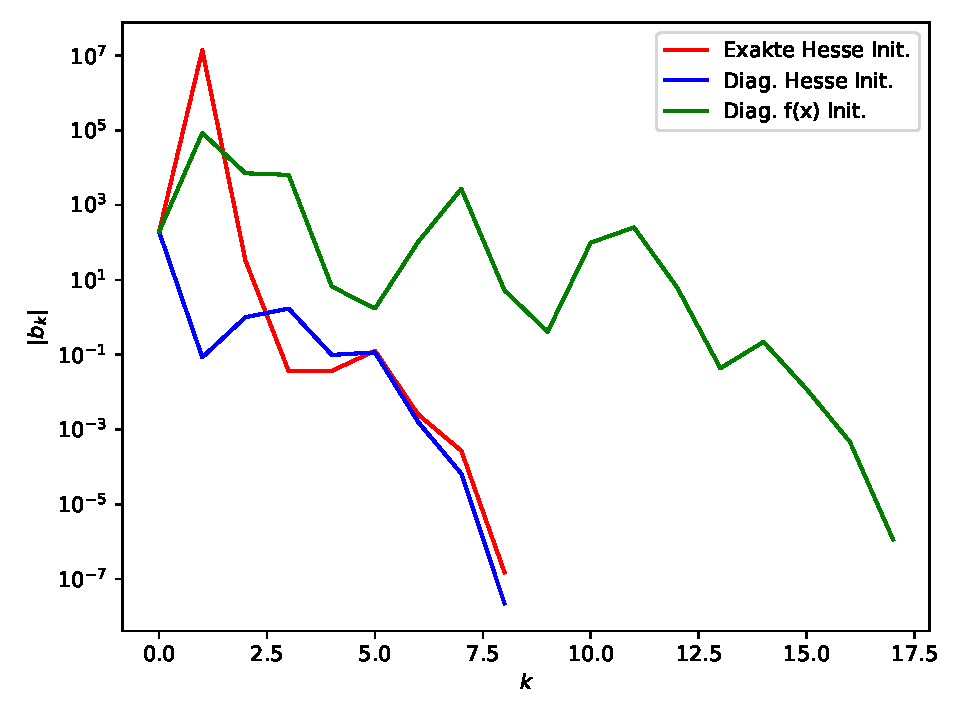
\includegraphics[width=0.45\textwidth]{A2/build/A2_l.pdf}
\caption{$|b_k|$ in Abhängigkeit vom Iterationschritt.}
\label{fig:1}
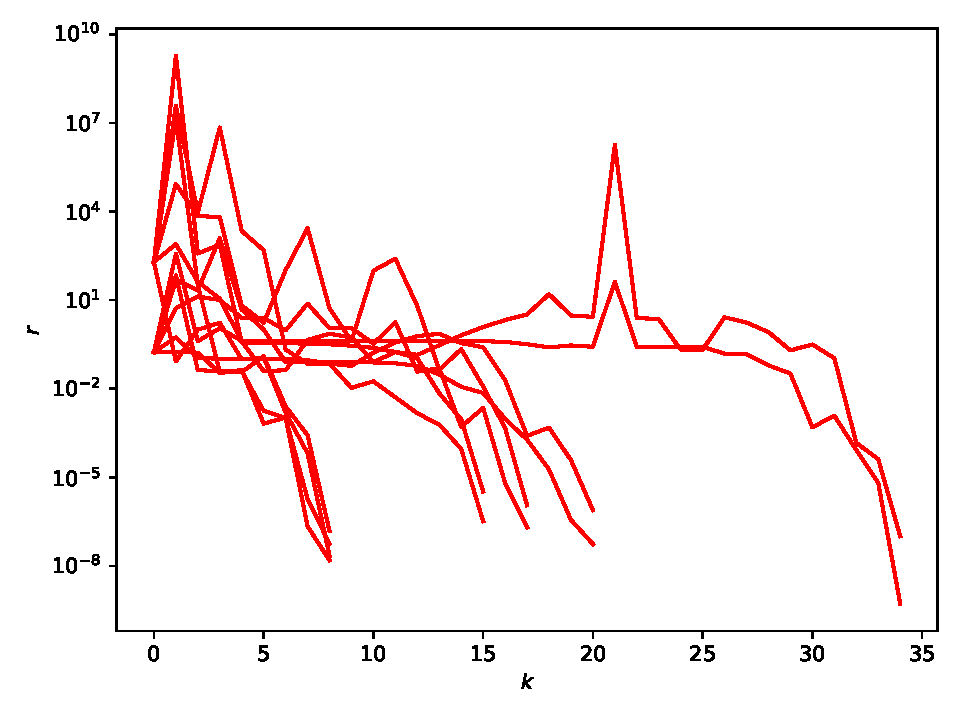
\includegraphics[width=0.45\textwidth]{A2/build/A2_lr.pdf}
\caption{Abweichung zum Minimum in Abhängigkeit vom Iterationschritt.}
\label{fig:2}
\end{figure}
%\subsection*{d)}
%Dieselben Verfahren aus Abschnitt \ref{sec:c} werden auf die Funktion \eqref{eq:2} durchgeführt.
%Für verschiedene Startvektoren
%\[
%\vec{x}_0 = \begin{pmatrix}
%1.5\\
%2.3
%\end{pmatrix},\begin{pmatrix}
%-1.7\\
%-1.9
%\end{pmatrix},\begin{pmatrix}
%0.5\\
%0.6
%\end{pmatrix}
%\]
%Die Gradientennorm und der Abstand zum Minimum
%\[
%\hat{\vec{x}}= \begin{pmatrix}
%
%\end{pmatrix}
%\]



%♥